\documentclass{article}
\usepackage{fancyhdr}
\usepackage{graphicx}
\usepackage{needspace}
\usepackage{amsthm,amssymb,amsmath}
\usepackage{fancyvrb}
\usepackage{tikz}
\usepackage{pgfplots}
\usepackage[section]{placeins}
\usepackage{float}
\usepackage{caption}
\usepackage{enumitem}
\usepackage{hyperref}
\usetikzlibrary{arrows, automata}

\pgfplotsset{compat=newest}
\renewcommand\qedsymbol{$\blacksquare$}
\pagestyle{fancy}

\fancyhf{}
\rhead{FALL 2019}
\lhead{CS440 - ASSIGNMENT 3 PART I}
\rfoot{\thepage}

\newtheorem{theorem}{Theorem}

\begin{document}

\begin{titlepage}
    \begin{center}
        \vspace*{1cm}
 
        \Huge
        \textbf{Assignment 3 Part I}
 
        \vspace{0.5cm}
        \LARGE
        Probabilistic Reasoning
 
        \vspace{1.5cm}
 
        \vspace{0.8cm}
  
        \Large
        Fall 2019\\
        Rutgers University\\
        CS440: Introduction to Artificial Intelligence\\
       	
       	\vspace{2cm}
        \large
        \textbf{Group Members} \\
        Joshua Rozenberg (jr922)\\
        JohnRobert Delos Santos (jad537)\\
   
    \end{center}
\end{titlepage}

\newpage
\pagenumbering{arabic}

\section{Problem 1}
Consider the following Bayesian network, where variables A through E are all Boolean valued. Note: there is a typo in the image, it should be P(A=true) = 0.2 instead of P(D=true) = 0.2.
\begin{figure}[H]
\centering
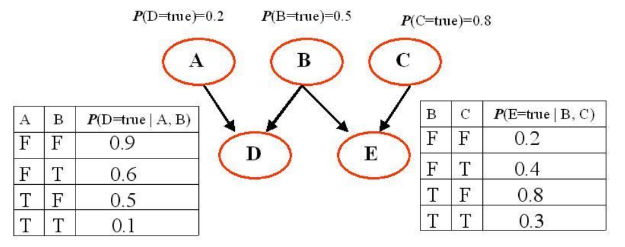
\includegraphics{images/1.png}
\end{figure}

\noindent
\textbf{a)} What is the probability that all five of these Boolean variables are simultaneously true?
\\\\
Decomposing the Bayesian network into conditional probabilities.
\\ $P(A,B,C,D,E) = P(A)P(D|A,B)P(B)P(E|B,C)P(C)$ 
\\ Then plug in the values for when all Boolean variables are true.\\
$P(A,B,C,D,E) = (0.2)(0.1)(0.5)(0.3)(0.8) = \textbf{0.0024}$
\\\\
\textbf{b)} What is the probability that all five of these Boolean variables are simultaneously false?
\\\\
We can use the decomposition above and the fact that $P(\neg A) = 1-P(A)$ to calculate the probability that all five of these Boolean variables are false.\\
$P(\neg A,\neg B,\neg C,\neg D,\neg E) =$\\
$P(\neg A)P(\neg D|\neg A,\neg B)P(\neg B)P(\neg E|\neg B,\neg C)P(\neg C)=$\\
$[1-P(A)][1-P(D| \neg A,\neg B)][1-P(B)][1-P(E| \neg B, \neg C)][1-P(C)]=$\\
$[1-0.2][1-0.9][1-0.5][1-0.2][1-0.8]=(0.8)(0.1)(0.5)(0.8)(0.2)=\textbf{0.0064}$
\\\\
\textbf{c)} What is the probability that A is false given that the four other variables are all known to be true?\\\\
$P(\neg A|B,C,D,E) = \frac{P(\neg A,B,C,D,E)}{P(\neg A,B,C,D,E)+P(A,B,C,D,E)}$\\
$P(A,B,C,D,E)=0.0024$\\
$P(\neg A,B,C,D,E)=P(\neg A)P(D|\neg A,B)P(B)P(E|B,C)P(C)=(0.8)(0.6)(0.5)(0.3)(0.8)=0.0576$\\
$P(\neg A|B,C,D,E) = \frac{0.0576)}{0.0576+0.0024}=\textbf{0.96}$
\newpage
\section{Problem 2}
\begin{figure}[H]
\centering
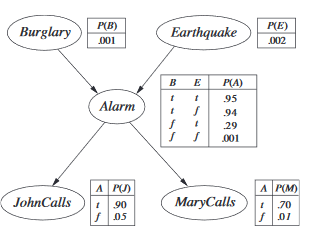
\includegraphics{images/2.png}
\end{figure}

\textbf{a)} Calculate $P(Burglary|JohnsCalls=true, MaryCalls=true)$ and show in detail the calculations that take place. 
\\\\
$Burglary = B, JohnCalls = J, MaryCalls = M, Earthquake = E, Alarm = A.$\\
To calculate $P(B|J,M)$, we need to find $P(B|J,M)$ and $P(\neg B|J,M).$ We will use inference by enumeration.\\\\
$P(B|J,M) = \alpha [P(B)\sum_{A} P(J|A)P(M|A) \sum_{E} P(A|B,E)P(E)]$\\
$=\alpha [P(B)\sum_{A} P(J|A)P(M|A) (P(A|B,E)P(E)+P(A|B,\neg E)P(\neg E))] $\\
$=\alpha [P(B)(P(J|A)P(M|A)(P(A|B,E)P(E)+P(A|B,\neg E)P(\neg E))$\\
$+P(J|\neg A)P(M|\neg A)(P(\neg A|B,E)P(E)+P(\neg A|B,\neg E)P(\neg E))]$\\
$=\alpha[(0.001)(0.9*0.7*(0.95*0.002+0.94*0.998)+0.05*0.01*(0.05*0.002+0.0.71*0.998))]$\\
$=\alpha 0.00059$\\\\
$P(\neg B|J,M) = \alpha [P(\neg B)\sum_{A} P(J|A)P(M|A) \sum_{E} P(A|\neg B,E)P(E)]$\\
$=\alpha [P(\neg B)\sum_{A} P(J|A)P(M|A) (P(A|\neg B,E)P(E)+P(A|\neg B,\neg E)P(\neg E))] $\\
$=\alpha [P(\neg B)(P(J|A)P(M|A)(P(A|\neg B,E)P(E)+P(A|\neg B,\neg E)P(\neg E))$\\
$+P(J|\neg A)P(M|\neg A)(P(\neg A|\neg B,E)P(E)+P(\neg A|\neg B,\neg E)P(\neg E))]$\\
$=\alpha[(0.999)(0.9*0.7*(0.29*0.002+0.001*0.998)+0.05*0.01*(0.71*0.002+0.0.999*0.998))]$\\
$=\alpha 0.0015$\\\\
$\alpha = \frac{1}{0.00059+0.0015} = 478.47$\\\\
$P(Burglary | JohnCalls = True, MaryCalls = True) = <P(B|J,M), P(\neg B|J,M)>$\\
$= < \textbf{0.282}, \textbf{0.718}>$\\
$ P(Burglary = True | JohnCalls = True, MaryCalls = True) = \textbf{0.282}.$
\newpage
\noindent
\textbf{b)} Suppose a Bayesian network has the form of a chain: a sequence of Boolean variables $X_1,...,X_n$ where $Parents(X_i)=\{X_{i-1}\}$ for $i=2,...,n.$ What is the complexity of computing $P(X_1|X_n=true)$ using enumeration? What is the complexity using variable elimination?
\\\\    
\textbf{Enumeration}\\
$$P(X_1|X_n=true)= \alpha \sum_{X_2,...,X_{n-1}} P(X_n = true|X_{n-1})P(X_{n-1}|X_{n-2})...P(X_3|X_2)P(X_2|X_1)P(X_1)$$\\
$$=\sum_{X_2,...,X_{n-1}} P(X_n = true|X_{n-1})P(X_{n-1}|X_{n-2})P(X_{x-2}|X_{x-3})...P(X_3|X_2)P(X_2|X_1)P(X_1)$$ \\\\
As we expand the summation, we can see that there will be $n-1-2+1$ or $n-2$ variables to take the sum over so overall, there will be $2_{n-2}$ terms. Every term size n will use $n-1$ multiplications. By combining the number of multiplications for each term and the number of terms, we get the runtime of enumeration as...
\begin{center}
$O(n2^{n-2})$
\end{center}
\textbf{Variable Elimination}\\
This method stores intermediate results to avoid re-computation and carries out summations right-to-left.\\
$$P(X_1|X_n=true)= \alpha \sum_{X_{n-1}} \sum_{X_{n-2}} P(X_{n-1}|X_{n_2})... \sum_{X_2} [P(X_3|X_2)P(X_2|X_1)P(X_1)]$$\\
$$= \alpha \sum_{X_{n-1}} \sum_{X_{n-2}} P(X_{n-1}|X_{n_2})... \sum_{X_3} P(X_4|X_3)f_{X_2}(X_3)$$
$$= \alpha \sum_{X_{n-1}} \sum_{X_{n-2}} P(X_{n-1}|X_{n_2})... \sum_{X_4} P(X_5|X_4)f_{X_3}(X_4)$$
If we continue this pattern to the end, we will see that there are $n-2$ summations in total. Because of the chain property and how variable elimination stores intermediate results, each summation will take a constant amount of additions so those are negligible to the overall runtime which will be...
\begin{center}
    $O(n)$
\end{center}

\newpage
\section{Problem 3}
\noindent
\textbf{a)} We constructed a Bayesian network based on the given description as such:\\
\noindent
\begin{figure}[H]
\centering
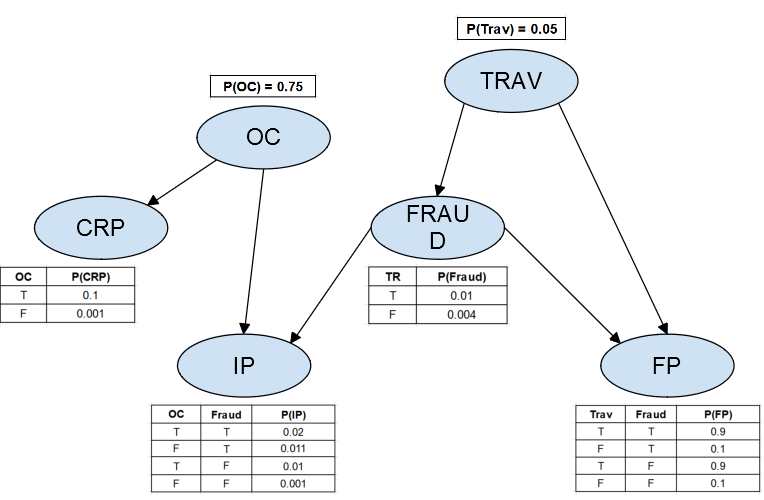
\includegraphics{images/3.png}
\end{figure}
\noindent
OC : card holder owns a computer or smart phone. \\
Fraud : current transaction is fraudulent. \\
Trav : card holder is currently travelling. \\
FP : current transaction is a foreign purchase. \\
IP : current purchase is an internet purchase. \\
CRP : a computer related purchase was made in the past week. \\
\newpage
\noindent
\textbf{b)} \\\textit{What is the prior probability (i.e., before we search for previous computer related purchases and before we verify whether it is a foreign and/or an internet purchase) that the current transaction is a fraud?}
\\\\
$P(Fraud) = P(Fraud | Trav = true) + P(Fraud | Trav = false)$\\
$P(Fraud) = 0.01 + 0.004 =$ \textbf{0.014} or \textbf{1.4\%}.
\\\\
\textit{What is the probability that the current transaction is a fraud once we have verified that it is a foreign transaction, but not an internet purchase and that the card holder purchased computer related accessories in the past week?}
\\\\
We can solve this using variable enumeration.\\
$$P(Fraud | FP, CRP, \neg IP)=$$
$$\alpha [\sum_{OC}P(OC)P(CRP|OC)P(\neg IP|OC,Fraud)][\sum_{Trav}P(Trav)P(Fraud|Trav)P(FP|Trav,Fraud)]$$
$$[\sum_{Trav}P(Trav)P(Fraud|Trav)P(FP|Trav,Fraud)] = $$
$$[P(Trav)P(Fraud|Trav)P(FP|Trav,Fraud)+P(\neg Trav)P(Fraud| \neg Trav)P(FP|\neg Trav, Fraud)] = $$
$$[(0.05)(0.01)(0.9)+(0.95)(0.004)(0.1)]$$
$$[\sum_{OC}P(OC)P(CRP|OC)P(\neg IP|OC,Fraud)] = $$
$$[P(OC)P(CRP|OC)P(\neg IP|OC, Fraud)+P(\neg OC)P(CRP|\neg OC)P(\neg IP|\neg OC, Fraud)] = $$
$$[(0.75)(0.1)(1-0.02)+(0.25)(0.001)(1-0.011)]$$
Replace both terms with their respective values to get:
$$P(Fraud | FP, CRP, \neg IP)= \alpha 0.0000612$$
Repeat the same process except with $\neg Fraud$.
$$P(\neg Fraud | FP, CRP, \neg IP)=$$
$$\alpha [\sum_{OC}P(OC)P(CRP|OC)P(\neg IP|OC,\neg Fraud)][\sum_{Trav}P(Trav)P(\neg Fraud|Trav)P(FP|Trav,\neg Fraud)]$$
$$[\sum_{Trav}P(Trav)P(\neg Fraud|Trav)P(FP|Trav,\neg Fraud)] = $$
$$[P(Trav)P(\neg Fraud|Trav)P(FP|Trav,\neg Fraud)+P(\neg Trav)P(\neg Fraud| \neg Trav)P(FP|\neg Trav, \neg Fraud)] = $$
$$[(0.05)(1-0.01)(0.9)+(0.95)(1-0.004)(0.1)]$$
$$[\sum_{OC}P(OC)P(CRP|OC)P(\neg IP|OC,\neg Fraud)] = $$
$$[P(OC)P(CRP|OC)P(\neg IP|OC, \neg Fraud)+P(\neg OC)P(CRP|\neg OC)P(\neg IP|\neg OC, \neg Fraud)] = $$
$$[(0.75)(0.1)(1-0.01)+(0.25)(0.001)(1-0.001)]$$
Replace both terms with their respective values to get:
$$P(\neg Fraud | FP, CRP, \neg IP)= \alpha 0.0103681$$
Solve for $\alpha$:
$$ \alpha = \frac{1}{0.0000612+0.0103681} = 95.88$$
$$ P(Fraud | FP, CRP, \neg IP) = \alpha <0.0000612, 0.0103681> = <\textbf{0.00587}, \textbf{0.99413}>$$
$$ P(Fraud = true | FP, CRP, \neg IP) = \textbf{0.00587} $$
$$ P(Fraud = false | FP, CRP, \neg IP) = 0.0103681 $$
\end{document}